Technology has made remarkable strides in recent years, revolutionizing the way we live, work, and connect with each other.
We can make life easier by having a personal assistant installed on a personal computer or mobile phone.
All the technologies require human interaction to operate, e.g.,\ computer, mobile, IoT devices, etc.
There are situations that humans can't provide proper interactions due to disabilities, lack of knowledge, and also for limited time as well.
A virtual personal assistant (VPA) is built with Machine Learning technologies such as Natural Language Processing (NLP), Speech Recognition, which can help in these situations by taking a voice command from the human and completing the tasks automatically.
For example, A virtual personal assistant (VPA) can be used to set a reminder, send email, know weather information, search information in Google, update to-do list, etc \cite{adheetee}.

\begin{figure}
    \centering
    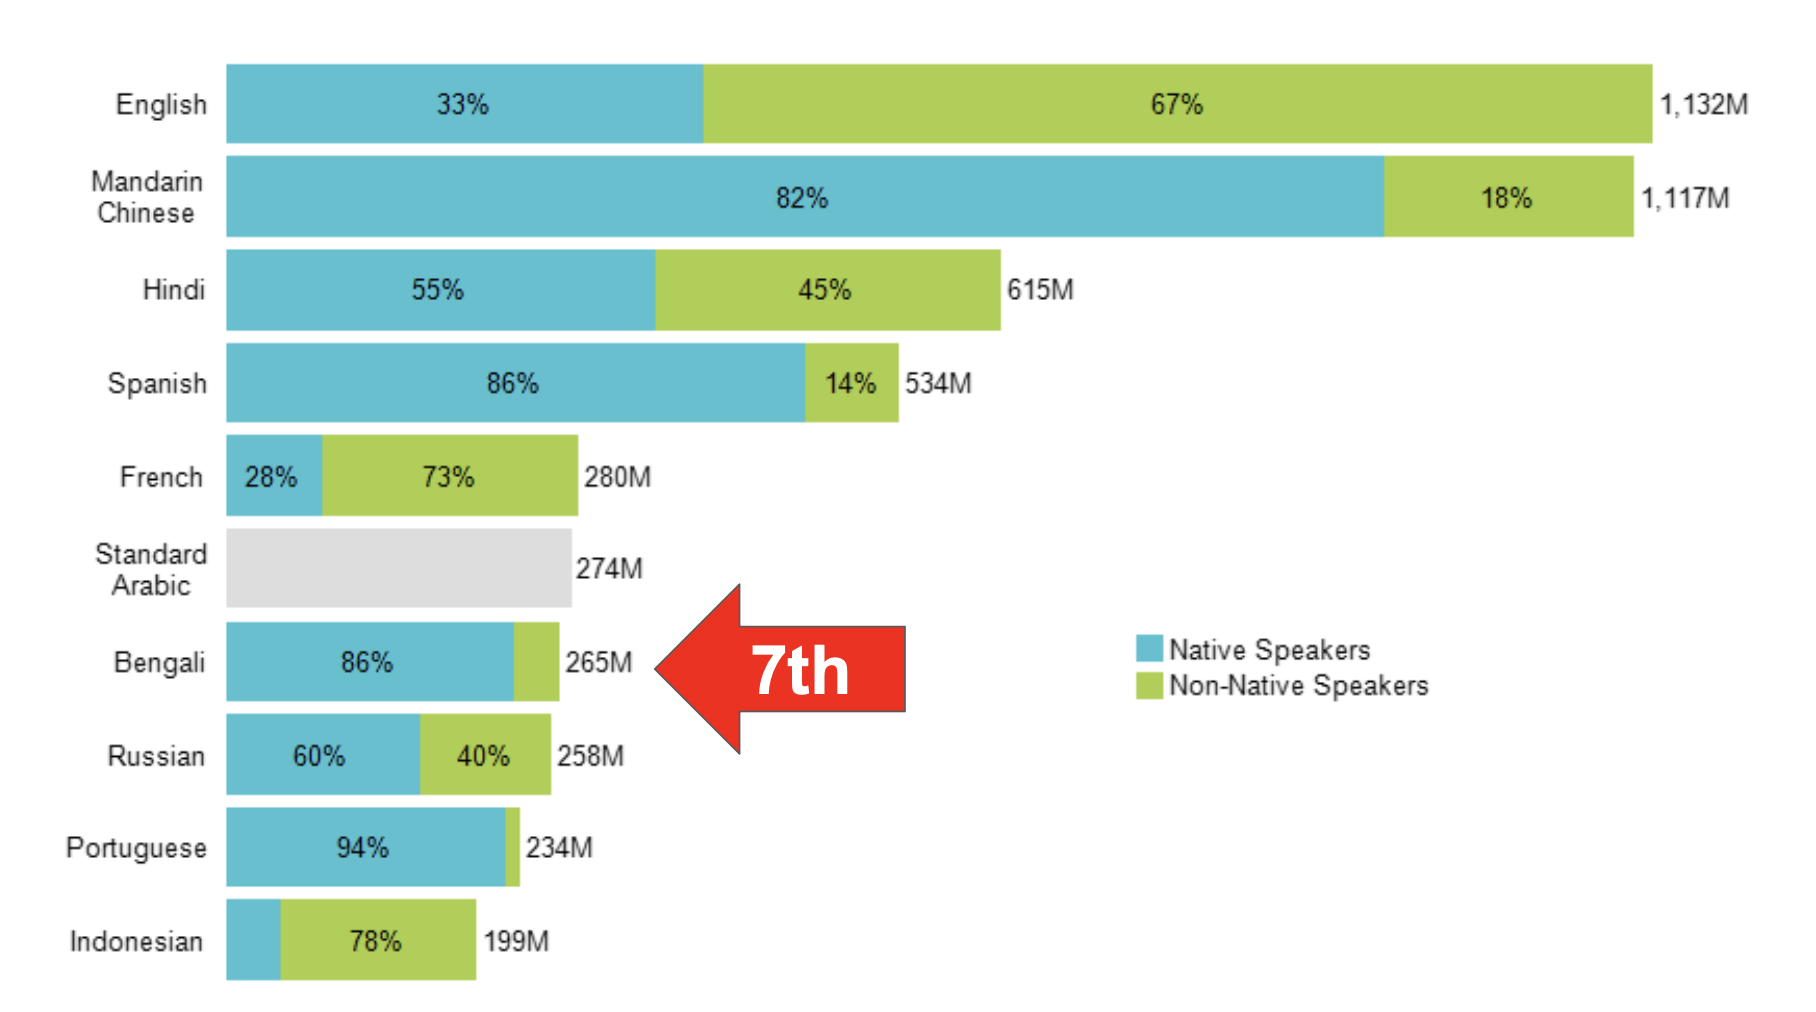
\includegraphics[width=0.4\textwidth]{top-speaking-world}
    \caption{Top Language Speaker in the World}\label{fig:top-speaking-world}
\end{figure}

\begin{figure}
    \centering
    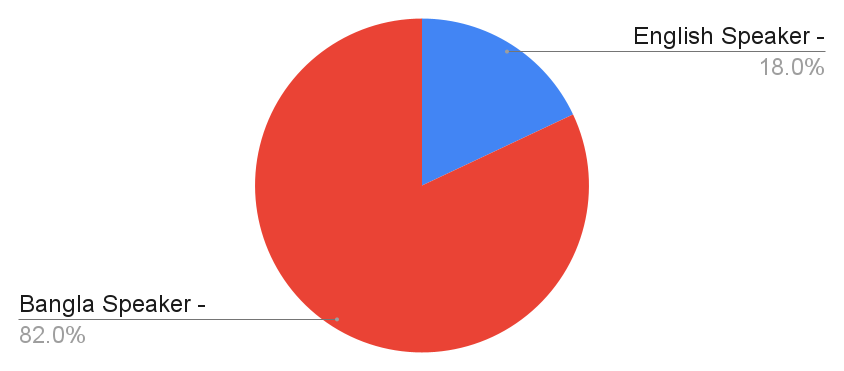
\includegraphics[width=0.4\textwidth]{top-speaking}
    \caption{Top Language Speaker in Bangladesh}\label{fig:top-speaking}
\end{figure}

Numerous works for the Virtual Personal Assistant (VPA) have been done for the English language throughout recent years.
Such as, Apple’s Siri\cite{siri}, Google’s Voice Actions\cite{google-mobile} and Google Now\cite{google-now}, Microsoft’s Bing Voice Search\cite{microsoft-tellme}, and Nuance’s Dragon Go! \cite{nuance-dragon} and Nina\cite{nuance-nina}, and many startup efforts like Speaktoit\cite{speaktoit}, and many more.

\begin{figure}
    \centering
    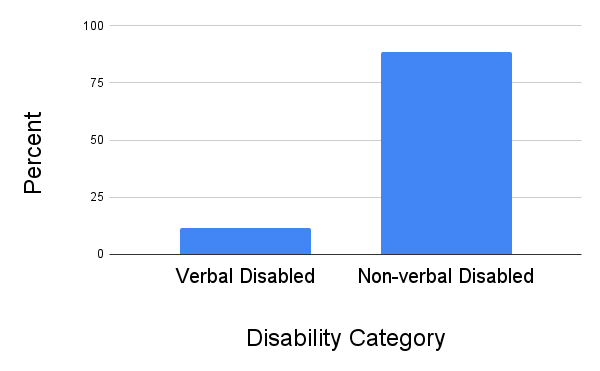
\includegraphics[width=0.4\textwidth]{verbal-disabled}
    \caption{Statistics for Categories in Disability in Bangladesh}\label{fig:verbal-disabled}
\end{figure}

\begin{figure}
    \centering
    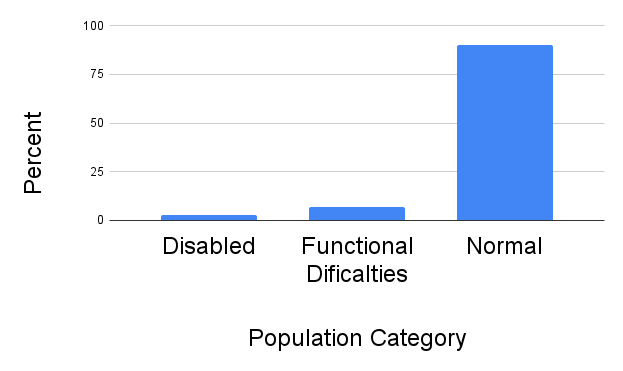
\includegraphics[width=0.4\textwidth]{population}
    \caption{Population distribution in Bangladesh in regard to Disability}\label{fig:polation}
\end{figure}

Bangla is the 7th most widely spoken language in the world, 272.7 million people (Figure \ref{fig:top-speaking-world}) around the world speak in Bangla \cite{mostspoken}.
Euro-monitor International reports only 18\% (Figure \ref{fig:top-speaking}) of the total population in Bangladesh can understand and speak English\cite{english-speaker-bangladesh}.
In addition, to that 25.34\% (literacy rate 74.66\% according to the Population and Housing Census 2022) of the total population is illiterate who cannot even read or write Bangla language\cite{litaracy-bangladesh}
According to Unicef Bangladesh, 2.8 percent (Figure \ref{fig:polation}) of the population and 1.7 per cent of children have at least one disability\cite{disabled-stats} in the country where Bengali is the primary language.
Among the disabled people, 11.43 (0.32 percent in the whole population) percent has limitations in speaking, and other 88.57 percent can at least speak (Figure \ref{fig:verbal-disabled}), but still they are away from technologies by other disabilities.

Although, very little work related to virtual personal assistant (VPA) had been done yet\cite{adheetee}.
We can't find any production grade virtual personal assistant (VPA) in the Bengali language as of today.

In this research, we propose a system with Speech to Text, Chatbot, and Text to Speech combined to develop a virtual personal assistant (VPA) that can help disabled (verbal) people to interact with technologies, save time for busy people by doing their technological tasks in no time wasted with just a voice command.
This virtual personal assistant will take voice commands, and based on that voice command it will do some actions like calling someone, interact with IoT devices, etc., and reply with the required information to answer the users' voice command.
In the other virtual personal assistant (VPA) we found that it lacks of personalizing for a specific person, but the solution to this problem is more required when we consider a disabled person.
Because they might not speak properly like other people, if we don't consider this problem, then it won't help them at all.
So, we introduce Reinforcement Learning (RL) for Speech-to-Text model to personalize user-specific voice characteristics.
%Researching personal assistants with reinforcement learning offers several compelling reasons.
%Firstly, reinforcement learning allows personal assistants to learn from user interactions and improve over time.
%This enables them to provide more personalized and effective assistance, tailoring responses to individual preferences and needs.
%Secondly, reinforcement learning empowers personal assistants to make autonomous decisions, enabling them to
%handle complex tasks and adapt to changing circumstances.
%This flexibility enhances their ability to assist users in various contexts.
%Moreover, reinforcement learning can help personal assistants optimize their performance by continuously learning and refining their strategies.
%This research can revolutionize the field, creating smarter, more capable personal assistants that offer enhanced user experiences.

%We have reviewed several papers that are related to our problem to some extent.
%We have seen how to develop a self-improving chatbot based on reinforcement learning \cite{rl-chatbot}, also we have seen information about developing to deploying about Siri Experience \cite{siri-experience}.
%Both of the paper has mentioned a different kind of information about building a solution for building a personal assistant.
%They are solving similar problems in different ways and in small or broader ways.
%By combining the experience of these papers we can build a new solution of our own to make a better solution in this area.
%The purpose of this work is to create a universal personal assistant that can understand human voice/texts and decide as it was set up before.
%We have a lot of chatbots or even personal Assistants like Siri \cite{siri}, Google’s Voice Actions \cite{google-mobile}, and many more.
%These are more of a chatbot, and you can do very basic actions with them like open an app, search for something on the web or in any app, etc.
%Our assistant will take a decision based on previously provided rules based on a given scenario.
%For example, if someone wants to have an appointment with me, if it is once configured to set an appointment then it would set it or discuss with me and the person to set a suitable time and date.
%So, this solution is not just a chatbot, it would be what we call an assistant.
